\documentclass[11pt,a4paper]{article}
\setcounter{secnumdepth}{6}

\usepackage{standalone}
\usepackage{graphicx}
\usepackage[font=footnotesize]{caption}
\usepackage[noadjust]{cite}
\usepackage[toc,page]{appendix}
\usepackage{hyperref}
\usepackage{fullpage}
\usepackage{amsmath}
\usepackage{sidecap}
\usepackage{caption}
\usepackage{subcaption}
\usepackage{minted}
\usepackage{framed}
\usepackage[colorinlistoftodos]{todonotes}
\usepackage{csquotes}
\usepackage{parskip} % Spaces between paragraphs

\usepackage{pgffor} % foreach loops!

\usepackage[acronym]{glossaries}


    \usepackage{adjustbox} % Used to constrain images to a maximum size 
    \usepackage{color} % Allow colors to be defined
    \usepackage{enumerate} % Needed for markdown enumerations to work
    \usepackage{geometry} % Used to adjust the document margins
    %\usepackage{amsmath} % Equations
    \usepackage{amssymb} % Equations
    \usepackage[mathletters]{ucs} % Extended unicode (utf-8) support
    % breaks things
    %\usepackage[utf8x]{inputenc} % Allow utf-8 characters in the tex document
    \usepackage{tcolorbox} % required to colour verbatim text
    \usepackage{fancyvrb} % verbatim replacement that allows latex
    \usepackage{grffile} % extends the file name processing of package graphics 
                         % to support a larger range 
    % The hyperref package gives us a pdf with properly built
    % internal navigation ('pdf bookmarks' for the table of contents,
    % internal cross-reference links, web links for URLs, etc.)
    %\usepackage{hyperref}
    \usepackage{longtable} % longtable support required by pandoc >1.10
    

    
%    
%    \definecolor{orange}{cmyk}{0,0.4,0.8,0.2}
%    \definecolor{darkorange}{rgb}{.71,0.21,0.01}
%    \definecolor{darkgreen}{rgb}{.12,.54,.11}
%    \definecolor{myteal}{rgb}{.26, .44, .56}
%    \definecolor{gray}{gray}{0.45}
%    \definecolor{lightgray}{gray}{.95}
%    \definecolor{mediumgray}{gray}{.8}
%    \definecolor{inputbackground}{rgb}{.95, .95, .85}
%    \definecolor{outputbackground}{rgb}{.95, .95, .95}
%    \definecolor{traceback}{rgb}{1, .95, .95}
%    % ansi colors
%    \definecolor{red}{rgb}{.6,0,0}
%    \definecolor{green}{rgb}{0,.65,0}
%    \definecolor{brown}{rgb}{0.6,0.6,0}
%    \definecolor{blue}{rgb}{0,.145,.698}
%    \definecolor{purple}{rgb}{.698,.145,.698}
%    \definecolor{cyan}{rgb}{0,.698,.698}
%    \definecolor{lightgray}{gray}{0.5}
%    
%    % bright ansi colors
%    \definecolor{darkgray}{gray}{0.25}
%    \definecolor{lightred}{rgb}{1.0,0.39,0.28}
%    \definecolor{lightgreen}{rgb}{0.48,0.99,0.0}
%    \definecolor{lightblue}{rgb}{0.53,0.81,0.92}
%    \definecolor{lightpurple}{rgb}{0.87,0.63,0.87}
%    \definecolor{lightcyan}{rgb}{0.5,1.0,0.83}
    
    % commands and environments needed by pandoc snippets
    % extracted from the output of `pandoc -s`
    \DefineVerbatimEnvironment{Highlighting}{Verbatim}{commandchars=\\\{\}}
    \definecolor{notebookgray}{rgb}{0.96, 0.96, 0.96}
    \newenvironment{InputVerbatim}
 {\VerbatimEnvironment
  \begin{tcolorbox}[colback=notebookgray,oversize,opacityframe=0]
  \begin{Verbatim}}
 {\end{Verbatim}\end{tcolorbox}}
 \newenvironment{StdOutVerbatim}
 {\VerbatimEnvironment
  \begin{tcolorbox}[colback=notebookgray,oversize,opacityframe=0]
  \begin{Verbatim}}
 {\end{Verbatim}\end{tcolorbox}}
 \newenvironment{OutputVerbatim}
 {\VerbatimEnvironment
  \begin{tcolorbox}[colback=notebookgray,oversize,opacityframe=0]
  \begin{Verbatim}}
 {\end{Verbatim}\end{tcolorbox}}


    
    
    \fvset{samepage=true}
   % \fvset{frame=single}
    % Add ',fontsize=\small' for more characters per line
    \newenvironment{Shaded}{}{}
    \newcommand{\KeywordTok}[1]{\textcolor[rgb]{0.00,0.44,0.13}{\textbf{{#1}}}}
    \newcommand{\DataTypeTok}[1]{\textcolor[rgb]{0.56,0.13,0.00}{{#1}}}
    \newcommand{\DecValTok}[1]{\textcolor[rgb]{0.25,0.63,0.44}{{#1}}}
    \newcommand{\BaseNTok}[1]{\textcolor[rgb]{0.25,0.63,0.44}{{#1}}}
    \newcommand{\FloatTok}[1]{\textcolor[rgb]{0.25,0.63,0.44}{{#1}}}
    \newcommand{\CharTok}[1]{\textcolor[rgb]{0.25,0.44,0.63}{{#1}}}
    \newcommand{\StringTok}[1]{\textcolor[rgb]{0.25,0.44,0.63}{{#1}}}
    \newcommand{\CommentTok}[1]{\textcolor[rgb]{0.38,0.63,0.69}{\textit{{#1}}}}
    \newcommand{\OtherTok}[1]{\textcolor[rgb]{0.00,0.44,0.13}{{#1}}}
    \newcommand{\AlertTok}[1]{\textcolor[rgb]{1.00,0.00,0.00}{\textbf{{#1}}}}
    \newcommand{\FunctionTok}[1]{\textcolor[rgb]{0.02,0.16,0.49}{{#1}}}
    \newcommand{\RegionMarkerTok}[1]{{#1}}
    \newcommand{\ErrorTok}[1]{\textcolor[rgb]{1.00,0.00,0.00}{\textbf{{#1}}}}
    \newcommand{\NormalTok}[1]{{#1}}
    
    % Define a nice break command that doesn't care if a line doesn't already
    % exist.
    \def\br{\hspace*{\fill} \\* }
    % Math Jax compatability definitions
    \def\gt{>}
    \def\lt{<}
    % Document parameters
    \title{2. Simulation}
    
    
    

    % Pygments definitions
    
\makeatletter
\def\PY@reset{\let\PY@it=\relax \let\PY@bf=\relax%
    \let\PY@ul=\relax \let\PY@tc=\relax%
    \let\PY@bc=\relax \let\PY@ff=\relax}
\def\PY@tok#1{\csname PY@tok@#1\endcsname}
\def\PY@toks#1+{\ifx\relax#1\empty\else%
    \PY@tok{#1}\expandafter\PY@toks\fi}
\def\PY@do#1{\PY@bc{\PY@tc{\PY@ul{%
    \PY@it{\PY@bf{\PY@ff{#1}}}}}}}
\def\PY#1#2{\PY@reset\PY@toks#1+\relax+\PY@do{#2}}

\expandafter\def\csname PY@tok@gd\endcsname{\def\PY@tc##1{\textcolor[rgb]{0.63,0.00,0.00}{##1}}}
\expandafter\def\csname PY@tok@gu\endcsname{\let\PY@bf=\textbf\def\PY@tc##1{\textcolor[rgb]{0.50,0.00,0.50}{##1}}}
\expandafter\def\csname PY@tok@gt\endcsname{\def\PY@tc##1{\textcolor[rgb]{0.00,0.27,0.87}{##1}}}
\expandafter\def\csname PY@tok@gs\endcsname{\let\PY@bf=\textbf}
\expandafter\def\csname PY@tok@gr\endcsname{\def\PY@tc##1{\textcolor[rgb]{1.00,0.00,0.00}{##1}}}
\expandafter\def\csname PY@tok@cm\endcsname{\let\PY@it=\textit\def\PY@tc##1{\textcolor[rgb]{0.25,0.50,0.50}{##1}}}
\expandafter\def\csname PY@tok@vg\endcsname{\def\PY@tc##1{\textcolor[rgb]{0.10,0.09,0.49}{##1}}}
\expandafter\def\csname PY@tok@m\endcsname{\def\PY@tc##1{\textcolor[rgb]{0.40,0.40,0.40}{##1}}}
\expandafter\def\csname PY@tok@mh\endcsname{\def\PY@tc##1{\textcolor[rgb]{0.40,0.40,0.40}{##1}}}
\expandafter\def\csname PY@tok@go\endcsname{\def\PY@tc##1{\textcolor[rgb]{0.53,0.53,0.53}{##1}}}
\expandafter\def\csname PY@tok@ge\endcsname{\let\PY@it=\textit}
\expandafter\def\csname PY@tok@vc\endcsname{\def\PY@tc##1{\textcolor[rgb]{0.10,0.09,0.49}{##1}}}
\expandafter\def\csname PY@tok@il\endcsname{\def\PY@tc##1{\textcolor[rgb]{0.40,0.40,0.40}{##1}}}
\expandafter\def\csname PY@tok@cs\endcsname{\let\PY@it=\textit\def\PY@tc##1{\textcolor[rgb]{0.25,0.50,0.50}{##1}}}
\expandafter\def\csname PY@tok@cp\endcsname{\def\PY@tc##1{\textcolor[rgb]{0.74,0.48,0.00}{##1}}}
\expandafter\def\csname PY@tok@gi\endcsname{\def\PY@tc##1{\textcolor[rgb]{0.00,0.63,0.00}{##1}}}
\expandafter\def\csname PY@tok@gh\endcsname{\let\PY@bf=\textbf\def\PY@tc##1{\textcolor[rgb]{0.00,0.00,0.50}{##1}}}
\expandafter\def\csname PY@tok@ni\endcsname{\let\PY@bf=\textbf\def\PY@tc##1{\textcolor[rgb]{0.60,0.60,0.60}{##1}}}
\expandafter\def\csname PY@tok@nl\endcsname{\def\PY@tc##1{\textcolor[rgb]{0.63,0.63,0.00}{##1}}}
\expandafter\def\csname PY@tok@nn\endcsname{\let\PY@bf=\textbf\def\PY@tc##1{\textcolor[rgb]{0.00,0.00,1.00}{##1}}}
\expandafter\def\csname PY@tok@no\endcsname{\def\PY@tc##1{\textcolor[rgb]{0.53,0.00,0.00}{##1}}}
\expandafter\def\csname PY@tok@na\endcsname{\def\PY@tc##1{\textcolor[rgb]{0.49,0.56,0.16}{##1}}}
\expandafter\def\csname PY@tok@nb\endcsname{\def\PY@tc##1{\textcolor[rgb]{0.00,0.50,0.00}{##1}}}
\expandafter\def\csname PY@tok@nc\endcsname{\let\PY@bf=\textbf\def\PY@tc##1{\textcolor[rgb]{0.00,0.00,1.00}{##1}}}
\expandafter\def\csname PY@tok@nd\endcsname{\def\PY@tc##1{\textcolor[rgb]{0.67,0.13,1.00}{##1}}}
\expandafter\def\csname PY@tok@ne\endcsname{\let\PY@bf=\textbf\def\PY@tc##1{\textcolor[rgb]{0.82,0.25,0.23}{##1}}}
\expandafter\def\csname PY@tok@nf\endcsname{\def\PY@tc##1{\textcolor[rgb]{0.00,0.00,1.00}{##1}}}
\expandafter\def\csname PY@tok@si\endcsname{\let\PY@bf=\textbf\def\PY@tc##1{\textcolor[rgb]{0.73,0.40,0.53}{##1}}}
\expandafter\def\csname PY@tok@s2\endcsname{\def\PY@tc##1{\textcolor[rgb]{0.73,0.13,0.13}{##1}}}
\expandafter\def\csname PY@tok@vi\endcsname{\def\PY@tc##1{\textcolor[rgb]{0.10,0.09,0.49}{##1}}}
\expandafter\def\csname PY@tok@nt\endcsname{\let\PY@bf=\textbf\def\PY@tc##1{\textcolor[rgb]{0.00,0.50,0.00}{##1}}}
\expandafter\def\csname PY@tok@nv\endcsname{\def\PY@tc##1{\textcolor[rgb]{0.10,0.09,0.49}{##1}}}
\expandafter\def\csname PY@tok@s1\endcsname{\def\PY@tc##1{\textcolor[rgb]{0.73,0.13,0.13}{##1}}}
\expandafter\def\csname PY@tok@sh\endcsname{\def\PY@tc##1{\textcolor[rgb]{0.73,0.13,0.13}{##1}}}
\expandafter\def\csname PY@tok@sc\endcsname{\def\PY@tc##1{\textcolor[rgb]{0.73,0.13,0.13}{##1}}}
\expandafter\def\csname PY@tok@sx\endcsname{\def\PY@tc##1{\textcolor[rgb]{0.00,0.50,0.00}{##1}}}
\expandafter\def\csname PY@tok@bp\endcsname{\def\PY@tc##1{\textcolor[rgb]{0.00,0.50,0.00}{##1}}}
\expandafter\def\csname PY@tok@c1\endcsname{\let\PY@it=\textit\def\PY@tc##1{\textcolor[rgb]{0.25,0.50,0.50}{##1}}}
\expandafter\def\csname PY@tok@kc\endcsname{\let\PY@bf=\textbf\def\PY@tc##1{\textcolor[rgb]{0.00,0.50,0.00}{##1}}}
\expandafter\def\csname PY@tok@c\endcsname{\let\PY@it=\textit\def\PY@tc##1{\textcolor[rgb]{0.25,0.50,0.50}{##1}}}
\expandafter\def\csname PY@tok@mf\endcsname{\def\PY@tc##1{\textcolor[rgb]{0.40,0.40,0.40}{##1}}}
\expandafter\def\csname PY@tok@err\endcsname{\def\PY@bc##1{\setlength{\fboxsep}{0pt}\fcolorbox[rgb]{1.00,0.00,0.00}{1,1,1}{\strut ##1}}}
\expandafter\def\csname PY@tok@kd\endcsname{\let\PY@bf=\textbf\def\PY@tc##1{\textcolor[rgb]{0.00,0.50,0.00}{##1}}}
\expandafter\def\csname PY@tok@ss\endcsname{\def\PY@tc##1{\textcolor[rgb]{0.10,0.09,0.49}{##1}}}
\expandafter\def\csname PY@tok@sr\endcsname{\def\PY@tc##1{\textcolor[rgb]{0.73,0.40,0.53}{##1}}}
\expandafter\def\csname PY@tok@mo\endcsname{\def\PY@tc##1{\textcolor[rgb]{0.40,0.40,0.40}{##1}}}
\expandafter\def\csname PY@tok@kn\endcsname{\let\PY@bf=\textbf\def\PY@tc##1{\textcolor[rgb]{0.00,0.50,0.00}{##1}}}
\expandafter\def\csname PY@tok@mi\endcsname{\def\PY@tc##1{\textcolor[rgb]{0.40,0.40,0.40}{##1}}}
\expandafter\def\csname PY@tok@gp\endcsname{\let\PY@bf=\textbf\def\PY@tc##1{\textcolor[rgb]{0.00,0.00,0.50}{##1}}}
\expandafter\def\csname PY@tok@o\endcsname{\def\PY@tc##1{\textcolor[rgb]{0.40,0.40,0.40}{##1}}}
\expandafter\def\csname PY@tok@kr\endcsname{\let\PY@bf=\textbf\def\PY@tc##1{\textcolor[rgb]{0.00,0.50,0.00}{##1}}}
\expandafter\def\csname PY@tok@s\endcsname{\def\PY@tc##1{\textcolor[rgb]{0.73,0.13,0.13}{##1}}}
\expandafter\def\csname PY@tok@kp\endcsname{\def\PY@tc##1{\textcolor[rgb]{0.00,0.50,0.00}{##1}}}
\expandafter\def\csname PY@tok@w\endcsname{\def\PY@tc##1{\textcolor[rgb]{0.73,0.73,0.73}{##1}}}
\expandafter\def\csname PY@tok@kt\endcsname{\def\PY@tc##1{\textcolor[rgb]{0.69,0.00,0.25}{##1}}}
\expandafter\def\csname PY@tok@ow\endcsname{\let\PY@bf=\textbf\def\PY@tc##1{\textcolor[rgb]{0.67,0.13,1.00}{##1}}}
\expandafter\def\csname PY@tok@sb\endcsname{\def\PY@tc##1{\textcolor[rgb]{0.73,0.13,0.13}{##1}}}
\expandafter\def\csname PY@tok@k\endcsname{\let\PY@bf=\textbf\def\PY@tc##1{\textcolor[rgb]{0.00,0.50,0.00}{##1}}}
\expandafter\def\csname PY@tok@se\endcsname{\let\PY@bf=\textbf\def\PY@tc##1{\textcolor[rgb]{0.73,0.40,0.13}{##1}}}
\expandafter\def\csname PY@tok@sd\endcsname{\let\PY@it=\textit\def\PY@tc##1{\textcolor[rgb]{0.73,0.13,0.13}{##1}}}

\def\PYZbs{\char`\\}
\def\PYZus{\char`\_}
\def\PYZob{\char`\{}
\def\PYZcb{\char`\}}
\def\PYZca{\char`\^}
\def\PYZam{\char`\&}
\def\PYZlt{\char`\<}
\def\PYZgt{\char`\>}
\def\PYZsh{\char`\#}
\def\PYZpc{\char`\%}
\def\PYZdl{\char`\$}
\def\PYZhy{\char`\-}
\def\PYZsq{\char`\'}
\def\PYZdq{\char`\"}
\def\PYZti{\char`\~}
% for compatibility with earlier versions
\def\PYZat{@}
\def\PYZlb{[}
\def\PYZrb{]}
\makeatother


    % Exact colors from NB
    \definecolor{incolor}{rgb}{0.0, 0.0, 0.5}
    \definecolor{outcolor}{rgb}{0.545, 0.0, 0.0}



    
    % Prevent overflowing lines due to hard-to-break entities
    \sloppy 
    % Setup hyperref package
%    \hypersetup{
%      breaklinks=true,  % so long urls are correctly broken across lines
%      colorlinks=true,
%      urlcolor=blue,
%      linkcolor=darkorange,
%      citecolor=darkgreen,
%      }
    % Slightly bigger margins than the latex defaults
    

\makeglossaries
\renewcommand*\abstractname{Summary}

% OUR COMMANDS
%~ 
%~ \newenvironment{pythoncode}%
%~ {\begin{framed}
%~ \begin{minted}{python}}%
%~ {\end{minted}
%~ \end{framed}}%

% http://www.tex.ac.uk/cgi-bin/texfaq2html?label=altabcr
\setcounter{MaxMatrixCols}{50}

% package name:
\newcommand{\means}{\texttt{MEANS}}
\newcommand{\pft}{\textit{p53}}
\newcommand{\py}{\texttt{python}}
\newcommand{\sympy}{\texttt{sympy}}
\newcommand{\plt}{\texttt{matplotlib}}
\newcommand{\mat}{\texttt{MATLAB}}
\newcommand{\eg}{\emph{e.g.}}
\newcommand{\ie}{\emph{i.e.}}

\newcommand{\sauliustodo}[2][]{\todo[color=cyan, #1]{\textbf{SL:} #2}}
\newcommand{\sisitodo}[2][]{\todo[color=yellow, #1]{\textbf{SF:} #2}}
\newcommand{\quentintodo}[2][]{\todo[color=red, #1]{\textbf{QG:} #2}}
\newcommand{\citationneeded}[2][]{\todo[color=brown, fancyline, #1]{\textbf{Citation Needed:} #2}}
\newcommand{\contrib}{\emph}
\begin{document}

\listoftodos
\newpage

\title{MEANS: a new python package for Moment Expansion Approximation, Inference and Simulation}
\author{Sisi Fan, Quentin Geissmann, Saulius Lukauskas.\\
\\	
\\
\\
\\
Supervised by Ann Babtie, Paul Kirk, Eszter Lakatos and Michael Stumpf\\
\\
\\
Theoretical Systems Biology Group,\\
Imperial College London
}
\date{\today}

\clearpage\maketitle
\thispagestyle{empty}
\newpage{}

\pagenumbering{roman}

\begin{abstract}
We present \means, a python package that provides stochastic modelling based on Moment Expansion Approximation (MEA), Linear Noise Approximation and Gillespie Stochastic Simulation Algorithm in an efficient and user-friendly way. Specifically for MEA, we have deployed scalar and three parametric moment closure methods in both univariate and multivariate forms. We also significantly improved MEA performance, which was a limiting factor in stochastic modelling.  In addition, the package also supports a collection of solvers and distance-based inference. To enhance usability and maintainability, we implemented modular design in the package with detailed documentation, as well as a series of interactive tutorials in IPython notebook format. In addition, our package supports SBML (Systems Biology Markup Language) standard for studying available biological systems. Apart from package development, we have conducted further analysis on MEA, and found higher using maximal moment order did not necessarily improve MEA accuracy. Moreover, we discovered that large parameter space could influence MEA accuracy and cause solver failure, which then might have led to incorrect inference based on MEA approximation. These limitations may provide insight into improvements of simulation and inference using MEA. We believe MEANS will a valuable package to study MEA and facilitate researchers to model non-linear kinetic systems. 
\end{abstract}

\tableofcontents

% our acronyms
\newacronym{ode}{ODE}{Ordinary Differential Equation}
\newacronym{mea}{MEA}{Moment Expansion Approximation}
\newacronym{lna}{LNA}{Linear Noise Approximation}
\newacronym{ssa}{SSA}{Gillespie Stochastic Simulation Algorithm}
\newacronym{cme}{CME}{Chemical Master Equation}
\newacronym{abc}{ABC}{Approximate Bayesian Computation}
\newacronym{sbml}{SBML}{Systems Biology Markup Language}
\newacronym{pypi}{PyPI}{the Python Package Index}

\newglossaryentry{maxord}
{
  name=max order,
  description={Maximal moment order. Max order always (regardless to the closure method) refers to the highest order of 
  moments present in an ODE system resulting from Moment Expansion Approximation. In other words, moment expansion is closed at Max order $\mathbf{+1}$
   },
  sort=max order
}
\gls{maxord}
\newpage{}
\printglossaries

\newpage{}
\pagenumbering{arabic}
\section{Introduction} \label{intro}

Most biological systems, such as cells, organisms, populations and ecosystems are intrinscaly complex and non-linear.
For this reason, some aspect of these systems are extremely difficult to understand and predict, both qualitatively and quantitatively\cite{klipp_systems_2013}.
Using explicit models to describe them provide an abstract and extensible framework which allows to infer the state of a system from experimental data.
In addition, models permit to make testable predictions on the behaviour of the system when parameters are modified.
In the last few decades, using mathematical representations of biological interactions has been an increasingly fruitful and wide aspect of biological research.
Many areas of biology, such as ecology, population biology and biochemistry,
use kinetic modelling to describe and understand temporal dynamics of their respective systems.

Deterministic modelling of dynamic systems generally involves listing
interacting agents (species) and decomposing a system in individual processes (\eg{} chemical reactions).
Processes are mathematically described with explicit rate parameters, and \glspl{ode} are used to express the change in the amount of species over time.
Generally, systems are assumed to be homogeneous, and the amount of each species is approximated as a continuous quantity.
This approach has been extremely useful for describing many systems, but it faces severe limitations when modelling small discrete quantities.
For instance, macromolecules in a cell can be present in a very small amount (less than hundred)\cite{ghaemmaghami_global_2003}.
In this situation, the assumptions of deterministic modelling may fail.
This has been shown to result in quantitative inaccuracy\cite{ale_general_2013}, and, in the worst cases, qualitatively erroneous predictions.


In order to overcome the limitations of deterministic modelling, stochastic modelling has been advanced as a solution.
It relies on \gls{cme}, which is a set of differential (or difference) equations providing an \emph{exact} description of a system\cite{kampen_stochastic_2011}.
Except for very simple systems, the \gls{cme} cannot be solved analytically.
However, it is possible to simulate single realisation of the Chemical Master Equation using \gls{gssa}.
If enough (generally several thousands), simulations are performed, very accurate estimations of the system can be obtained.
Despite extensive effort on increasing the efficiency of such simulations, either by describing new algorithms, or by improving implementations,
they remain too slow for certain problems.
In particular, when trying to infer biological parameters from experimental data, according to an explicit model,
it is necessary to perform many simulations.
In extreme cases, such as for \gls{abc}\cite{toni_approximate_2009}, a very large number of simulations are necessary in order to obtain an 
accurate posterior distributions for parameters.
Therefore, for parameter inference, stochastic simulations are unfortunately critically slow and can rarely be used, even for relatively simple systems.

In order to overcome performance limitations of stochastic simulations whist providing accurate enough results, approximations have been used.
\Gls{lna}, for instance, approximates the \gls{cme}
by taking in account only the means (first order raw moments), and the variances and covariances (second order central moments)\cite{komorowski_bayesian_2009}.
This method is often limited to cases where the amount of each species is large and systems consist of first order reactions
(such as  $a \rightarrow b$, but not $a + c  \rightarrow b$)\cite{ale_general_2013}.

Another approach aims to expand the \gls{cme} by expressing central moments in terms of second or third order central moments\cite{gillespie_moment-closure_2009, gomez-uribe_mass_2007}.
Recently, this concept has been generalised to expand the \gls{cme} up to any arbitrary moment order\cite{ale_general_2013}.
This method, \gls{mea}, has shown very promising results, but has not been investigated in detail yet.

To model the changes in concentrations using \gls{mea}, higher order moments are required to express the lower order moments
(\ie{} the $i^{th}$ moment depends on the $(i+1)^{th}$ moment).
This makes the expressions for moments infinitely long, and, obviously, the \glspl{ode} impossible to solve analytically. In order to make the approach computable, a strategy for stopping the
expansion of moment terms by approximating (closing) higher order moments is necessary.

In the original publication\cite{ale_general_2013}, higher order moments were assumed to be zero. 
This approach is elegant mathematically, but may not necessarily be the best one.
If, instead, an assumption is made on the distribution of the species numbers, it is possible
to express any moment in terms of parameters of this distribution\cite{milner_moment_2011}.
Therefore, instead of closing moment expansion with an absolute (scalar) value, the higher order moments can be expressed in
terms of distribution parameters such as mean and variance, which are moments of order one and two.

In principle, \emph{a priori} information on the system can help to decide what type of closure is appropriate for a given system.
Preliminary investigation of this ``parametric moment expansion closure'' in the context of MEA has been shown to be promising\cite{lakatos_preparation_2014}.

\subsection{The Aim of the Project}

\gls{mea} being a very recent development, no comprehensive public implementation has been made available to the community yet.
A \mat{} implementation was developed by the authors of the original publication. A \py{} implementation of \gls{mea} together with \gls{lna}, simulation and parameter inference routines, has also been attempted by the previous year's MSc students\cite{babtie_moment_2013}.
However, both implementations are still prototypical and not ready to be made available to the general public.
 
The aim of our work was to improve and extend existing tools in order to provide a comprehensive publication-ready implementation of \gls{mea}.
We provide \means{}, a \py{} package for Moment Expansion Approximation, iNference and Simulation. 
Here we build on top of the existing functionality in the aforementioned \py{} implementation, aiming to restructure it to make it easier to manage, as well as document it better. 
We also implement the support moment expansion closure using Normal, Log-Normal and Gamma distributions in addition to the original scalar (or zero) closure. Similarly, we provide \gls{gssa} implementation in the package as well as support for different \gls{ode} solvers and additional visualisation functionality.

In the report herein, we explain the decisions that drove the design of the package.
Then, we describe the new restructured structure of the code that improves it's maintenabilty.
Afterwards, we provide some examples of intended use in the form of tutorials to the illustrate the usability and the scope of \means.
We then demonstrate how we managed to considerably improve the scalability and performance of the system during the development.
We then go on and use this newly-created package to critically assess \gls{mea}, and address potential limitations.
Finally, we attach the exhaustive documentation for future maintainers and users to the appendix of this document.

\newpage
\section{Approach to Software Design}
\label{sec:design_considerations}

Our software development has been heavily inspired by the Agile methodology\cite{_manifesto_????}.
Agile methodology has been established as an alternative to the traditional waterfall method which views requirements gathering, software design and implementation as a linear process.
In contrast to this traditional view, agile methodology centres around iterative approach to software development, and aims to minimise the cost caused by problems along the way.

The key principles of this methodology have been neatly summarised by Kelly Waters\cite{_what_????}:

\blockquote{
    [The] characteristics that are common to all agile methods, and the things that I think make agile fundamentally different to a more traditional waterfall approach to software development [\ldots] are:
    
    \begin{enumerate}
        \item Active user involvement is imperative
        \item The team must be empowered to make decisions
        \item Requirements evolve but the timescale is fixed
        \item Capture requirements at a high level; lightweight \& visual
        \item Develop small, incremental releases and iterate
        \item Focus on frequent delivery of products
        \item Complete each feature before moving on to the next
        \item Apply the 80/20 rule
        \item Testing is integrated throughout the project lifecycle -– test early and often
        \item A collaborative \& cooperative approach between all stakeholders is essential
    \end{enumerate}
}

While these principles may sound very vague, they capture the recommendations based on years of trial-and-error on software development in the industry, and generally act as good guidelines to follow for projects with short deadlines.

\subsection{Requirements Gathering}
\label{sec:requirements-gathering}
One of the key parts of any project is the requirements gathering process -- no amount of skill or hard work will help if the work is misdirected.
Naturally, we took great interest in getting these requirements right.

Capturing requirements at ``\emph{at a high level}" was important for this project since the temptation to discuss about low-level implementation before gathering requirements was great.
These discussions are often constraining the requirements with the implementation details, while ideally we wanted the requirements to influence the implementation decisions, and not the other way around.

The easiest way to keep the requirements in a high level was to limit the discussion to a set of scenarios of usage.
These scenarios are commonly referred to \emph{user stories} and usually follow the template: ``As (some user type, \eg{} \emph{a scientist)} I would like to (some action, \eg{} \emph{perform these calculations}) because (optionally, the reason for this use case)".
The first part of this relatively free-form story gives a view of the potential user base of the software.
For instance researchers and undergraduate students may have different requirements.
The second part provides a set of important use cases for the problem.
Finally, the third part assesses the relative importance of each of the use cases.

We were able to write down four representative user stories, listed below:
\begin{enumerate}

    \item \emph{As a researcher studying biological systems, I would like to perform a variety of simulations, with different parameter sets, and compare the results of these simulations.}

    \item \emph{As a researcher studying the approximation method, I would like to be able to compare the changes to the approximation quality, when the approximation parameters (\ie{} the closure method) are changed.}

    \item \emph{As a researcher studying biological systems, I would like to be able to infer the set of parameters of the model given the data, but this idea is still not very popular in my field and I am not sure if it is feasible.}

    \item \emph{As a systems biologist, I am used to dealing with multiple data formats, and I am computer-savvy enough to adapt to any format implemented by the software, as long as it is reasonably simple.}
\end{enumerate}

The pattern emerging from these use cases was that our project software should be designed to be an intermediate step in some larger data analysis process, and should not try to limit the remaining steps of the process.
For instance, the \emph{comparison} process in the first two user stories could not be clarified in more detail, because the techniques are employed there in a very \emph{ad-hoc} fashion.

Similarly, the fourth user story indicates that the origin of the input data and its format are undefined.
Therefore the software needed be general enough to support multiple input formats, or have a simple enough format allowing researchers to convert their data to.

This observation encouraged us to move away from the traditional command-line application model for this software, which was assumed for the previous implementation\cite{babtie_moment_2013}.
In our opinion, flexibility of command-line applications comes at the expense of simplicity -- we have all seen really flexible applications that have a list of parameters that is too long for a newcomer to comprehend.
Similarly, command-line applications create an artificial gap between the data processing and data analysis step, \ie{} writing and reading file output, which can be reduced if the application was returning the data in the format that can readily be used to investigate the data.

In order to satisfy these requirements, we designed \means{} package with flexibility and interactivity in mind. 
The flexibility requirement impacted certain decisions made while structuring the package, which are further described in \autoref{sec:package}.
Interactivity of the package has been ensured by coding specific behaviours for the IPython interactive python environment \cite{perez_ipython:_2007}.

\subsection{Package Structure}
\label{sec:package}

In order to make the code easier to maintain and manage, we have divided \means{} package into nine different smaller submodules, each responsible for a different part of the system.
We have paid particular attention in making all the necessary features importable using the pythonic shorthand \verb"from means import *", 
as to ensure it is simple enough to use \means{} in interactive environments where it might be uncomfortable to deal with modularity explicitly.

The nine submodules in \means{} and their respective role are listed below:
\begin{enumerate}
    \item \verb"means.core" -- the core functionality, such as the definitions of key classes
    \item \verb"means.approximation" -- implementations of the \gls{lna} and \gls{mea} approximation methods.
    
    \item \verb"means.simulation" -- implementation of various \gls{ode} solving algorithms.
    \item \verb"means.inference" -- implementation of parameter inference methods
    \item \verb"means.io" -- implementation of input and output routines
    \item \verb"means.util" -- utility functions used across the modules, internal to the package
    \item \verb"means.tests" -- various tests for the package functionality, hidden from the user by default
    \item \verb"means.examples" -- definitions of example models that are used throughout tutorials, needs to explicitly be imported by the user.
    \item \verb"means.pipes" -- optional module providing wrappers for pipeline support
\end{enumerate}

Each submodule is described in detail below.

\subsubsection{{\tt means.core} -- core classes used within all other packages}
% If you are editing this, please also edit src/means/core/__init__.py docstring
% to keep the two consistent
This package stores the common classes that are used within all of the other means sub-packages.

The module exposes the descriptor classes, such as \verb"Descriptor",
\verb"VarianceTerm", \verb"Moment" and
\verb"ODETermBase" that are used to describe the types of trajectories generated,
as well as certain terms in the ODE equations.

Similarly, both the \verb"StochasticProblem" and
\verb"ODEProblem" classes that are used in stochastic and deterministic simulations respectively are exposed by this module.

Finally, the \verb"Model" class, which provides a standard interface to describe a biological model, and can be thought to be the center of the whole package, is also implemented here.

The tutorial \autoref{sec:modelling_using_means} provides a comprehensive review on how these objects could be used in combination to model biological systems in \means{}.

\subsubsection{{\tt means.approximation} -- approximation methods for biological models}

The approximation submodule implements \gls{lna} and \gls{mea} methods for biological systems encoded in \means{} format.

The approximation package is itself split into two sub-packages, one for each of the two approximation methods.
This keeps specific routines in separate modules, thus avoiding \gls{lna} and \gls{mea} implementations namespace polluting each other.
This also provides a clear path for future developers to implement new approximation methods -- simply creating another sub-package.

Despite being in different packages, both approximation methods inherit from the same base class, intuitively named \verb"ApproximationBaseClass".
This base class defines the common interface all approximation methods; namely, the dependency on \verb"Model" and public \verb"run()" method that implements the mathematics and returns a \verb"ODEProblem" object that can be simulated.
This common interface is required for any pipeline using the approximation methods to be method-agnostic.
In other words, we want the pipeline to be able to perform the approximation in exactly the same way, regardless of whether \gls{lna} or \gls{mea} was used. 
It is easy to see how this design pattern increases the code maintainability and compatibility as well: not only the future maintainer will have a clear template to follow for implementing an approximation method, but it will also be immediately compatible with all the code using the approximations already.

In order to keep the usage of the \means{} convenient in interactive environments, we also provide shorthand methods \verb"mea_approximation" and \verb"lna_approximation", that perform the instantiation of the approximation object and the generation of expressions using it in one step.

The usage of these approximation methods is described in exhaustive detail in the tutorial \autoref{sec:modelling_stochastic_dynamics}.

\subsubsection{{\tt means.simulation} -- stochastic and deterministic simulation routines}
\label{sec:package_structure:simulation}

The next submodule in the list provides the routines for performing deterministic and stochastic simulations.
These simulations are performed via \verb"Simulation" and \verb"SSASimulation" classes defined in this sub-module.

Unlike the approximation package, the simulation routines could not share the same interface, as they have different inputs -- a stochastic simulation needs \verb"StochasticProblem" that provides the stoichiometry matrix as well as hazard functions to simulate stochastically, while the deterministic simulation routine requires an \verb"ODEProblem" object that is essentially a collection of ordinary differential equations.
Nevertheless, the classes still share the same interface, providing a \verb"simulate_system()" method which in turn generates a set of \verb"Trajectory" objects, to keep them consistent.

Also unlike the approximation submodule, we deliberately do not provide the convenience methods for performing simulations and force the user to create the \verb"Simulation" objects herself. 
Firstly, the convenience functions for simulations would have to have a lot of parameters, in order to be as flexible as the explicit creation of the simulator objects. 
This is a non-issue for the approximation objects, whose heavy-lifting function takes zero parameters, so all of the complexity is in the constructor parameters only.
Secondly, due to the way we perform numerical evaluations, subsequent uses of the same \verb"Simulation" object are much cheaper than the very first use of it which has to precompile the numeric routines.
This point is further discussed in \autoref{sec:evaluating_expressions_efficiently} as well as illustrated in the tutorial \autoref{sec:reuse_of_simulation_objects}. 
Providing a shorthand for these functions would encourage the users to use the non-efficient path, as reuse of simulation objects would not be possible, and therefore we chose not to do this.

The tutorial chapter \autoref{sec:simulation} provides a complete guide of this submodule.

\subsubsection{{\tt means.inference} -- parameter inference methods}
% Change src/means/inference/__init__.py if you are modifying this
This part of the package provides utilities for parameter inference.
Parameter inference will try to find the set of parameters which
produces trajectories with minimal distance to the observed trajectories.

Different distance functions are implemented (such as functions minimising the sum of squares error
or functions based on parametric likelihood), but it is also possible to use customised distance functions.

The package provides support for both inference from a single starting point (\verb"Inference")
or inference from random starting points (\verb"InferenceWithRestarts").

Advance plotting functionality for inference results and the parameter space is also provided by the package, which is used extensively in the sections of the report covering the parameter inference (\eg{} \autoref{sec:results:inference}). 

A full user guide for using this submodule is provided in the tutorial \autoref{sec:parameter_inference}.

\subsubsection{{\tt means.io} -- reading and writing of \means-specific objects}
% change src/means/io/__init__.py if you are changing this
The module implements common methods to serialise and deserialise objects in \means.
Namely the module provides functions \verb`means.io.dump` and  \verb`means.io.load` that would
serialise and deserialise the said objects into YAML format\cite{_official_????}.
These serialised representations can be written to or read from files with the help of
\verb`means.io.to_file` and \verb`means.io.from_file` functions.
% this is not in __init__.py, but is required for report
The YAML format has been chosen due to it's ability to balance human and machine readability. 
Some examples of the YAML serialised objects can be seen in the tutorial section covering this package, i.e. \autoref{sec:input_output}, particularly \autoref{sec:human_readable_serialisation}.

%this is in __init__.py again
For the user's convenience, the said methods are also attached to all serialisable objects,
e.g. \verb`means.core.Model.from_file()` method would allow the user to read a \verb`means.core.Model` object from file directly.

%also in __init__.py
We do not provide any convenience functions for binary serialisation of the object, because \verb`pickle` package,
which is in the default distribution of Python, has no problems of performing these tasks on \means objects. 
We recommend using \verb`pickle`, rather than \verb`means.io` whenever fast serialisation is preferred to human
readability.

% still in __init__.py
Finally, this module also provides support for the input from SBML files\cite{hucka_systems_2003}.
If the \verb`libsbml` is installed in the user's system and has the appropriate python bindings, the function \verb`means.io.read_sbml` can be used to parse the files in SBML format
to \verb`means.core.Model` objects. See example usage in \autoref{sec:reading_models_from_files}.

\subsubsection{{\tt means.util} -- utility functions used within the package}
% change src/means/util/__init__.py if you're changing this
This package contains helper functions that did not fit into any other packages.
These functions include helper functions for common operations when dealing with \verb`sympy`,
as well as functions that help with memorisation of CPU intensive function results.

These functions are designed to be package-specific.
The users of the software are generally discouraged to use any of these functions.

\subsubsection{{\tt means.tests} -- ensuring the working implementation}
The tests package contains, rather unsurprisingly, the tests for our implementation.
Our approach to testing is described in \autoref{sec:testing}

\subsubsection{{\tt means.examples} -- example models used in the documentation}
The examples package contain a set of toy models used in the documentation.
The models included with the package are:
\begin{itemize}
    \item a sample Michaelis-Menten kinetics model as in \cite{ale_general_2013};
    \item Dimerisation model, also in \cite{ale_general_2013};
    \item P53 model, described in \cite{ale_general_2013} and in tutorial \autoref{sec:modelling_using_means} of this document;
    \item HES1 model, based on the description in \cite{ale_general_2013};
    \item A textbook example of Lotka-Volterra dynamics \cite{billard_lotka-volterra_1977}.
\end{itemize}

These example models are designed to help us to illustrate important concepts of the package in the documentation, but are otherwise independent from the package, and therefore need to be imported separately.
The user of the software is nevertheless encouraged to experiment with these toy models.

\subsubsection{{\tt means.pipes} -- convenience functions for data pipelines}
The \emph{pipes} submodule provides convenience wrappers around the main functionalities in \means{} that allow seamless integration with \verb"luigi" package for pipeline support\cite{_luigi_????}.

This submodule has allowed us to break down the figures needed for our report into a set of smaller tasks. 
Once the dependancies of each of these tasks were encoded, \verb"luigi" package could then ensure these tasks are performed in the correct order, parallelise the tasks that are mutually exclusive, even among multiple computers, and not run the tasks that have already been finished twice.

This essentially allowed us to specify the figures needed for report in a very high level fashion, in turn allowing us to be more flexible with them, as well as to be certain that we do not have to do the same work twice.

More about this can be found in SL's individual report and the documentation available in the appendix \autoref{sec:documentation}.

\subsection{Testing}
\label{sec:testing}

``Test early and often" has now become one of the the catch-phrases associated with \emph{agile} software development (see \autoref{sec:design_considerations}). 
This catchy sentence gives a twofold advice: integrate testing as early as possible to your development lifecycle, and perform as many tests as possible.

Starting testing early is of particular importance because the cost of discovering problems increases exponentially with effort put into the process.  
For instance, we were quite happy to allow some extra time fixing an unexpected problem with our code early on in the project, but we would be seriously stressed if some riddle popped up as we are writing this report, due to the deadline approaching. 
Similarly, in some scenarios such problem might just invalidate all the previous hard work done earlier on.

In other words, early testing allows to specify the requirements
    \footnote{We use the word \emph{requirements} in a slightly different sense in this section compared to the one in \autoref{sec:requirements-gathering}. 
    Here the term \emph{requirements} is used from the code perspective and is synonymous to \emph{specification}, \emph{contract}, \emph{interface} of the code, whereas the same term in the previous section refers to the overall requirements of the software, which may be captured by a combination of these code-specific requirements described here.} 
for the code early on and allow us to ensure they continue to be satisfied as we progress through the development lifecycle. 


We were in particularly good position to start testing early, due to the work done by the people working on this project previously. 
As a starting point, we started by the output from this project as the true behaviour of the system, encode this requirement in the code, and find an automatic way of checking that this is still the case. 
We call these tests \emph{regression} tests as they are designed to validate that we have not introduced any new faults to the system,
essentially establishing a baseline performance of it.
We chose to use all of the examples given in the previous year's group report as a good starting point of our regression tests.

In order to \emph{test often}, as suggested by the same slogan mentioned earlier, we fired up an continuous integration server using Jenkins platform\cite{_jenkins_????}. The main purpose of this continuous integration server was to run our whole test suite after each commit to a github repository, and notify us if there are problems with it. 
This way we can eliminate the human factor and ensure that the tests are really run often and completely and therefore ensure the continuous compliance with the specification.

As the software evolved, the regression tests were slowly phased out into unit tests for particular parts of the software. The main difference between the two types of the tests is that the regression tests test a large part of the system for preservation of a certain function, while unit tests focus on some small part of the system and explicitly tests it's behaviour independently. Given a large enough coverage of unit tests, we can be reasonably certain that the overall system also works fine, and thus eliminate the regression tests (which are often very slow to run). To illustrate this better, picture a GC content counting algorithm for some DNA sequence. 
A regression test (sometimes also called functional test) would run the algorithm on whole DNA sequence and check that the overall output is, say, 60\%. 
Unit tests would only test a small subset of the system, for instance, it could check that given a particular window of DNA, the overall GC count is correctly computed in that window. Similarly, it could check that given a couple of counts obtained from such windows, they are averaged correctly and so on. 

It is possible to imagine that if combination of these unit tests are all fine, the functional test result should also be fine, so we are not losing any information by replacing these bulky tests with more fine-grained ones. It is also not hard to picture how this fine-graining could help spot problems with code faster, which is the main reason of these transitions. 

In the end, of the project, 66\% of the lines of our code had at least some test associated with it, with most of the tests lacking from the methods associated with plotting and reporting the results back to the user, that have been tested by other means. Namely by automatically re-compiling the tutorials you in the \autoref{examples} and checking if there were any problems or inconsistencies.
\newpage{}
\section{Installation, Example Usage and Tutorial} \label{examples}
In this section, we illustrate the main functionality of \means{} by in a short tutorial.
Please, note that the tutorial instructions below are auto-generated from the interactive tutorial in the IPython notebook format, and therefore paper might not be the best medium for this content.

For the readers convenience, we also provide an online read-only version of this tutorial, available at \url{http://msc.bc.ic.ac.uk:2712/}. 

If the reader has access to a working python installation and \means{} source-code,
fully operational interactive version of the tutorials could be run directly in the IPython notebook, by typing:

\begin{InputVerbatim}
cd examples/Tutorials
ipython notebook
\end{InputVerbatim}

A new browser window with the tutorial notebooks should open automatically.

\sauliustodo[inline]{Add screenshots}

\subsection{Installation}

In order to install \means{} package, one must first make sure all external dependancies such as \verb"sundials" libraries \cite{hindmarsh_sundials_2005} are installed. 
Our \verb"README.txt" file located in the \verb"src" directory of the codebase provides some guidance on how to do this.

Once the dependancies are all accounted for, the development version of the \means{} package can be installed by navigating to the \verb"src" directory of the codebase, and issuing the install command via a standard \py{} package installation tool \verb"pip":

\begin{InputVerbatim}
pip install -e .
\end{InputVerbatim}

This command should fetch and install all the dependancies of \means{} as well as the package in the development mode (specified by the \verb"-e" flag). 
Troubleshooting information is provided in the same \verb"README.txt" file.

Note that in order to be able to use the \means{} package to its full potential, the user is encouraged to install the latest version of  IPython notebook\cite{perez_ipython:_2007} as well.

Once the code is released to public, \means{} could be immediately pushed to \gls{pypi}, what would allow to shorten the installation procedure to just \verb"pip install means" command.

{   % These brackets are very important, btw.

    % IPython notebook likes to define their own colours...
    % And who could blame them.
    
    \definecolor{orange}{cmyk}{0,0.4,0.8,0.2}
    \definecolor{darkorange}{rgb}{.71,0.21,0.01}
    \definecolor{darkgreen}{rgb}{.12,.54,.11}
    \definecolor{myteal}{rgb}{.26, .44, .56}
    \definecolor{gray}{gray}{0.45}
    \definecolor{lightgray}{gray}{.95}
    \definecolor{mediumgray}{gray}{.8}
    \definecolor{inputbackground}{rgb}{.95, .95, .85}
    \definecolor{outputbackground}{rgb}{.95, .95, .95}
    \definecolor{traceback}{rgb}{1, .95, .95}
    % ansi colors
    \definecolor{red}{rgb}{.6,0,0}
    \definecolor{green}{rgb}{0,.65,0}
    \definecolor{brown}{rgb}{0.6,0.6,0}
    \definecolor{blue}{rgb}{0,.145,.698}
    \definecolor{purple}{rgb}{.698,.145,.698}
    \definecolor{cyan}{rgb}{0,.698,.698}
    \definecolor{lightgray}{gray}{0.5}
    
    % bright ansi colors
    \definecolor{darkgray}{gray}{0.25}
    \definecolor{lightred}{rgb}{1.0,0.39,0.28}
    \definecolor{lightgreen}{rgb}{0.48,0.99,0.0}
    \definecolor{lightblue}{rgb}{0.53,0.81,0.92}
    \definecolor{lightpurple}{rgb}{0.87,0.63,0.87}
    \definecolor{lightcyan}{rgb}{0.5,1.0,0.83}
    
    % Tutorials go here
    \input{autogenerated-tutorials}
}   % make sure to put them above this line


\newpage{}
\section{Results and Discussion} \label{results}



\subsection{Performance}\label{performance}
\sauliustodo{I think this should be moved somewhere earlier in the report as it justifies the pretext of our work}
The temporal dynamics of a molecular system can be described by the \acrfull{cme}\citationneeded{CME reference}.
\acrfull{gssa}\cite{gillespie_general_1976} simulates these stochastic dynamics directly returning a set of individual trajectories for a list of particles observed.
In order to obtain accurate estimates of the average dynamic within a population of cell (\ie{} the mean dynamics), it is however necessary to perform multiple (often more than $10^4$) simulations.
Despite recent efforts \cite{niemi_efficient_2011,dittamo_optimized_2009,komarov_accelerating_2012} to provide fast implementation of this algorithm, computation remains extremely expensive. \quentintodo{Do you know the Big-Oh complexity?} This time-complexity is a limiting factor in downstream analysis techniques,
for instance parameter inference that often requires repetition of these experiments for a large set of parameter values.

This particular limitation led to the development of approximations such as \acrfull{lna}\cite{komorowski_bayesian_2009} and \acrfull{mea}\cite{ale_general_2013} which model the mean behaviour directly, without evaluating the individual particle behaviours, and therefore can perform in a more realistic time.

Since the main driving force for development of these approximation algorithms is the potential reduction of the time taken to perform the  analysis, it is paramount to make the implementation as efficient as possible.

In this section, we explore the implementation factors that influence the runtime of the algorithm, and describe the optimisations done to increase the performance of it. In particular, we show that symbolic computations can be limiting the algorithm and explain the techniques used to optimised them. We also quantify the increase of performance  and show that it is several order of magnitudes better than the original \mat{} implementation.
In addition, we explore other limiting factors we have less control of, such as the choice of \gls{ode} solver, and discuss their potential implications to the analysis of biological systems.

\subsubsection{Optimising \acrlong{mea}}


\gls{mea} involves derivation of a system \gls{ode}s from a model.
This procedure\cite{ale_general_2013}, involves lengthy symbolic calculations.
Even for very simple models (\eg{} three species, five reactions), they cannot be realised manually.
The number equations in the generated \gls{ode} system, for a model with $s$ species and up to moments of order $o$ can be estimated by the following equation: 
\quentintodo[inline]{Does not make sense for 3 species, and 2nd-order moments (3+2-2 choose 3) - 1 = 0}
\begin{displaymath}
    \text{Number of equations} = {{s + o - 2} \choose {s}} - 1
\end{displaymath}
As a consequence, the complexity of the calculation is predicted to increase exponentially with the number of species in the system and the maximal order of moments. \quentintodo[inline]{Add an example numbers illustrating this: "For instance, for a 2-species system ...."}

%In order to perform symbolic computations, we have used \sympy{} \cite{sympy_development_team_sympy:_2014}; a \py{} implementation of
%the symbolic computation routines.

In order to increase the scalability of the method, we have identified significant bottlenecks in our procedures using \py{} profiling tools. We have then attempted to iteratively remove these bottlenecks one by one. Figure~\ref{fig:mea_speed} shows the cumulative effects of different optimisations.

\quentintodo[inline]{Explain why no original python performance line, reduce the detail in caption, make it more evident it is log-normal}


\begin{figure}[tbh]

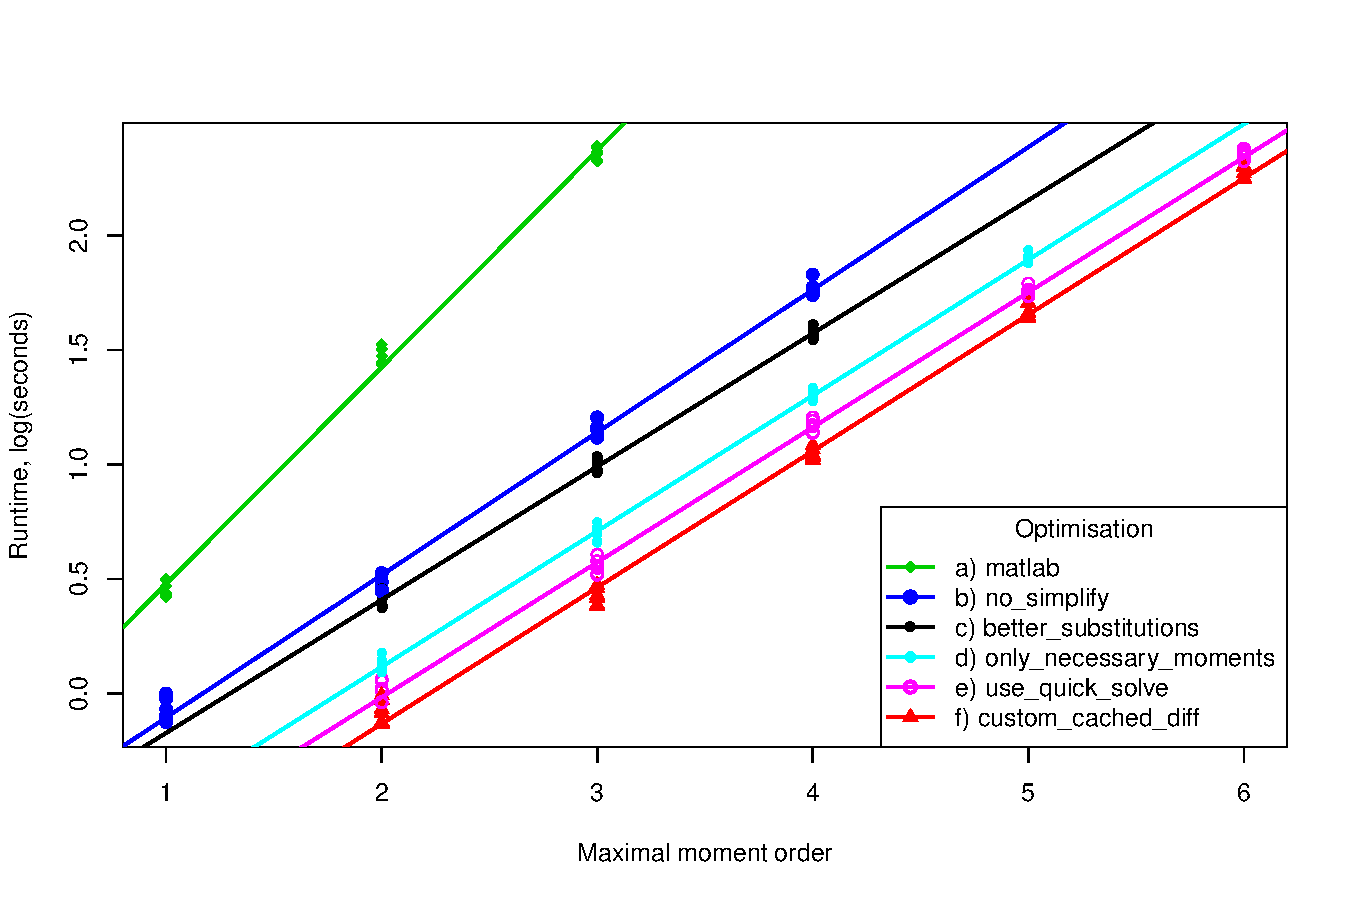
\includegraphics[width=1.0\textwidth{}]{../figure_mea_speed/mea_speed.pdf}
\caption{\emph{Cumulative performance improvement of symbolic calculations resulting from optimisation}.
The processing time for computing log-normal closure on \pft{} model with different maximal moment orders were measured for original Matlab implementation (a) and different optimisations (b$-$f).
In a first place, the calls to \texttt{sympy.simplify()} where removed (b). 
Then, \texttt{sympy.xreplace()} was used instead of \texttt{sympy.substitute()} (c). 
Generating an $(n-s) \times (n_2-s + 1)$ matrix (d), as opposed to an $(n-s) \times (n-s + 1)$ one, also increase speed (see main text).
Implementing a simplified equation solver instead of using \texttt{sympy.solve()} also resulted in a significant speed-up (e). Finally, caching (memorisation) \texttt{sympy.diff()} allowed even better performance.
The time complexity appears exponential ($O(2^n)$, where $n$ is the maximal moments order) in every case, 
Interestingly, the slopes between, a ($0.95$) and c ($0.58$), and b ($0.62$) and c were significantly different ($p-value <10^{-15}$ and $p-value = 3 \times 10^{-4}$, respectively; t-test on the slopes of the linear regression). 
No significant difference was found between the slopes of the subsequent optimisations (c$-$f). 
However, the intercepts were significantly smaller between each consecutive optimisations after c) ($p-value < 10^{-6}$ for all; t-test on the intercepts of the linear regression).
Nine replicates were performed on the same CPU. For optimisation c$-$f, values corresponding to maximal order moments lower than two were removed because of the inherent inaccuracy in measuring very short durations}
\label{fig:mea_speed}
\end{figure}

\quentintodo[inline]{Simplify this, move out the specific details to your individual report, it is enough to give just the overview here.}

The first step involved removing the expression simplification heuristic.
In the original code\footnote{both from the publication and last year's MSc project}, the right-hand-side equations were simplified in order to produce shorter text file results.
However, this was slow and did not benefit subsequent simulations and inference.
For large expressions, simplification had also had an large memory footprint and was likely to fail.
This optimisation significantly improved the scalability of the method (see fig.~\ref{fig:mea_speed}, b).

The next bottleneck was the choice of substitution functions.
As a part of \gls{mea}, it is necessary to replace raw moment symbols by expressions depending on central moments.
Performing substitution can be done using the \texttt{substitute()} function from \sympy, but this is designed to substitute expressions by other expressions.
In most cases, we only had to substitute atomic symbols by expression.
For this purpose, the  \texttt{xreplace()} function was a much more appropriate alternative which resulted in a better scalability (see fig.~\ref{fig:mea_speed}, c).

In the original implementation, a matrix of central moment expression of size $(n-s) \times (n-s + 1)$ is directly generated when the default closure is applied.
However, when using a parametric closure, a matrix of size $(n_2-s) \times (n_2-s + 1)$, where $n_2={{s+o-2 \mathbf{+1}} \choose {s}} -1$, was generated.
The $n_2 - n$ rows corresponding to higher-order moments have then to be deleted.
In contrast, out implementation generates a $(n-s) \times (n_2-s + 1)$ matrix regardless of the closure method.
In addition to improve code readability, consistency and flexibility \footnote{see QG's individual report}, this improved overall performance (fig.~\ref{fig:mea_speed}, d) for cases where closure is applied while keeping the default closure computation fast.

Another simple way to improve computation time was to remove calls to the function \texttt{solve()} which was only used in straightforward cases (\eg{} solving: $a + 2b = c$ for $a$).
It was therefore much more efficient (fig.~\ref{fig:mea_speed}, e) to use simple arithmetic to find solution.

Finally, partial derivation of expression over several variables and order is extensively performed during the approximation.
Generally, these type of differentiations can be simplified several differentiation of first order:
\begin{equation}
\frac{\partial{} ^ 2 f(x,y)}{\partial x \partial y}  =
\frac{\partial{} \frac{\partial{} f(x,y)}{\partial x}}{\partial y} =
\frac{\partial{} \frac{\partial{} f(x,y)}{\partial{} y}}{\partial{} x}
\end{equation}
One advantage, is that, when needing to calculate two derivatives such as:  $\frac{\partial{} ^ 2 f(x,y)}{\partial{} x \partial{} y}$ and $\frac{\partial{} ^ 2 f(x,y)}{\partial{} x^2}$, 
one can precompute $\frac{\partial{} f(x,y)}{\partial{} x}$ and use it for both calculation.
In our implementation, we have use a procedure known as \emph{memorisation} which, briefly, permits to store the results of a function call in an associative array.
Then, the next time this function is called with the same arguments, it will return the stored results instead of recomputing it.
This also resulted in an overall performance improvement (fig.~\ref{fig:mea_speed}, f).

In conclusion, reorganising, profiling and rewriting the code resulted in incremental significant performance improvements of symbolic computations in \means{} compared to the original \mat{} code.
For instance, with the same \pft{} system and closure method, 
we predict that computation up to \gls{ode}s up $8^{th}$ order will take 44 minutes with \means{} and as much as 128 days with the original implementation.\quentintodo{Add a number saying how long it would have taken for the first iteration of optimisation as well.}
These improvement have allowed us to explore the performance of MEA in higher depth, and will hopefully contribute to make \gls{mea} realistically usable for systems with more species and reactions.

\subsection{Moment Expansion Closure}

In \gls{mea} the temporal derivative of each central moment of order $n$ is expressed in terms of moment of order $n+1$.
For this reason, it is necessary to ``close'' the expansion by providing a closed form for the higher order moments.
In the original work \cite{ale_general_2013}, higher order central moments are assumed null. 
This is a strong and not necessarily valid assumption. 

Parametric probability distribution can be used to express moment of arbitrary orders. 
For instance, a multivariate normal distribution is parametrised only by means (\emph{i.e } first order raw moment)
and a covariance matrix (\emph{i.e.} second order central moments). 
As a consequence, it is possible to express any arbitrary moment from means, variances and covariances. 
A promising area of research involves closing moment expression by parametric forms of highest order central moments instead
of assuming them to be null.
Preliminary work \todo{cite Eszter, unpublished} suggests that using a parametric distributions for \gls{mea}
In addition, Ale \emph{et al.} predicted that higher maximal moment order would necessarily result in better approximation \cite{ale_general_2013}.
closure could greatly improve approximation.
The dramatic improvement in performance compared to the original code and implementation of parametric closures made it possible to verify both of these claims.

Figure~\ref{fig:max_order_and_closure_on_distance} shows the effect of increasing maximal moment order and different type of closures.
The \pft system, with parameters from \cite{ale_general_2013}, was investigated.
For normal and scalar closures, as expected, the approximation globally improves with maximal moment order (reduced distance to \gls{gssa}).
However, for 7$~{th}$ order, the scalar closure had an increased distance, and solving normal closures \gls{ode}s was not possible.
Note that for even maximal moment orders, normal and scalar are rigorously equal.
This is expected since normal distribution is symmetrical (\emph{i.e.} odd central moments are always zero).

In contrast, log$-$normal closures are fitting to the ground through trajectory well for maximal moment order of three,
but the approximation gets less and less accurate for higher maximal order moments.
A deeper look at the trajectories indicate that, in this latter case,
oscillations are damping too quickly (fig.~\ref{fig:max_order_and_closure_on_distance}b).
Interestingly for even maximum moment order log$-$normal closures generated \gls{ode}s which,
despite our efforts, could not be numerically solved.

Finally, for this system and parameter set, univariate and multivariate distributions closures were very similar.
For other systems such as \emph{hes1}, it was advantageous to model covariance (data not show).

This results indicates that the quality of the approximation depends both on the type of closure, on the maximal moment order and on their interaction. This makes it difficult to \emph{a priori} define which closure and maximal moment order should be used for a given system.

\begin{figure}

\includegraphics[width=1.0\textwidth]{../pipeline/task-output/FigureP53Summary/FigureP53Summary-pdf-7.pdf}
\includegraphics[width=1.0\textwidth]{../pipeline/task-output/FigureP53Simple/FigureP53Simple-pdf-7.pdf}
%~
\caption{\emph{Effect of different closure methods and maximal moment order on simulation accuracy}.
The \pft system was modelled using \gls{mea} with five types of closure and for maximal moment order up to seven.
Resulting trajectories were all compared to an average of 5000 \gls{gssa} simulations using sum of square distance (a).
Distance is in log scale.
For illustration purposes, complete trajectories of a single species (\pft) for max order three and seven are shown (b).
Black lines indicate the average of \gls{gssa} simulations. Missing points (b) and lines (a) indicate solver failure
TODO(see failure section.)}

\label{fig:max_order_and_closure_on_distance}
\end{figure}

\subsection{Inference}
Inference uses a distance method to infer parameter values by exploring the parameter space and comparing the distance between inferred system behaviour with experimental data. 

In order to study the performance of the inference method in \means, we used "sum of squares" distance method and p53 model. 
Due to the lack of experimental concentrations of the species, the averaged concentration change through time from $5000$ \gls{gssa} are used as the observed trajectories. 
With full variability for all the parameters in the p53 model, and starting values equal to the values from \cite{gillespie_general_1976}, it is expected that the inference method would return the same values as the starting values. 
To visualise how the system explored the multi-dimensional parameter space, we studied the cross-section for all possible pairs of parameters. \sisitodo{find the 7 dimensional figure} 
Unexpectedly, trajectories simulated with the true parameter values are distant from the \gls{gssa} trajectories, forcing the system to follow the distant gradient and infer incorrect parameter values. This result implies inference method is may not infer the right parameter set. 

To confirm if the inference method can find the global minima, we recorded the inferred parameter values using one pair of parameters at a time for all possible pairs of parameters, and used these values as the starting values to re-generated the distance landscape (see Figure 5 \sisitodo{check if it's the right number}). 
Here, we explicitly allow $c_2$ and $c_6$ values to vary, but keep other parameter values the true values, because $c_2$ and $c_6$ with variability in their values are able to produce an almost perfect match with the \gls{gssa} trajectories of all species (data not shown). 
If the inference method was correct, the starting point in the distance landscape would already have a low distance, and the end point should overlap with the starting point, i.e. the true values of $c_2$ and $c_6$.
However, the resulting distance landscape figures and trajectories for each species clearly indicate that the starting point is not the global minima, because: Firstly, the trajectories in the distance landscape shows the starting point can be distant from the minima; Secondly, the possible range for $c_6$, despite the maximal order for \gls{mea}, is mostly more than 10 times larger than the true value; Thirdly, the trajectories for all the species in the p53 model sometime demonstrate misfit between the optimal trajectory obtained from inference and the "observed trajectory" from \gls{gssa}. 

Based on these results, we can conclude that the inference method here is inaccurate.
\begin{figure}
\centering
    \begin{subfigure}
    \includegraphics[width=0.2\textwidth]{{../pipeline/task-output/SampleMultidimensionInferenceFigure/SampleMultidimensionInferenceFigure-pdf-1-scalar-True-90.0_0.002_1.704_1.1_0.93_0.96_0.7822-ode15s--90.0_0.002_1.704_1.1_0.93_0.96_0.7822-sum_of_squares-5000}.pdf}
    \end{subfigure}
    \begin{subfigure}
    \includegraphics[width=0.2\textwidth]{{../pipeline/task-output/SampleMultidimensionInferenceFigure/SampleMultidimensionInferenceFigure-pdf-2-scalar-True-90.0_0.002_1.704_1.1_0.93_0.96_0.7822-ode15s--90.0_0.002_1.704_1.1_0.93_0.96_0.7822-sum_of_squares-5000}.pdf}
    \end{subfigure}
    \begin{subfigure}

    \includegraphics[width=0.2\textwidth]{{../pipeline/task-output/SampleMultidimensionInferenceFigure/SampleMultidimensionInferenceFigure-pdf-3-scalar-True-90.0_0.002_1.704_1.1_0.93_0.96_0.7822-ode15s--90.0_0.002_1.704_1.1_0.93_0.96_0.7822-sum_of_squares-5000}.pdf}
    \end{subfigure}
    \begin{subfigure}
    \includegraphics[width=0.2\textwidth]{{../pipeline/task-output/SampleMultidimensionInferenceFigure/SampleMultidimensionInferenceFigure-pdf-4-scalar-True-90.0_0.002_1.704_1.1_0.93_0.96_0.7822-ode15s--90.0_0.002_1.704_1.1_0.93_0.96_0.7822-sum_of_squares-5000}.pdf}
    \end{subfigure}
    \begin{subfigure}
    \includegraphics[width=0.2\textwidth]{{../pipeline/task-output/SampleMultidimensionInferenceFigure/SampleMultidimensionInferenceFigure-pdf-5-scalar-True-90.0_0.002_1.704_1.1_0.93_0.96_0.7822-ode15s--90.0_0.002_1.704_1.1_0.93_0.96_0.7822-sum_of_squares-5000}.pdf}
    \end{subfigure}

\caption{\emph{Distance landscape at different maximal orders for p53 model.} In the landscape, the warmer the colour, the more distant the inferred trajectories are from the \gls{gssa} trajectories. 
The \gls{gssa} trajectories are generated using the new parameter values labelled as \emph{start}. Among seven parameters, only the values for $c_2$ and $c_6$ are inferred, with starting values inferred from inference using the true values.} 
\label{fig:parameter_inference_landscape}
\end{figure}

\begin{figure}
\centering
    \begin{subfigure}
    \includegraphics[width=0.6\textwidth]{{../pipeline/task-output/FigureInferenceStartEndSSA/FigureInferenceStartEndSSA-1-scalar-c2-1.7040-c6-0.7822}.pdf}
    \end{subfigure}
    \begin{subfigure}
    \includegraphics[width=0.6\textwidth]{{../pipeline/task-output/FigureInferenceStartEndSSA/FigureInferenceStartEndSSA-2-scalar-c2-1.7040-c6-0.7822}.pdf}
    \end{subfigure}
    \begin{subfigure}    
    \includegraphics[width=0.6\textwidth]{{../pipeline/task-output/FigureInferenceStartEndSSA/FigureInferenceStartEndSSA-3-scalar-c2-1.7040-c6-0.7822}.pdf}
    \end{subfigure}
    \begin{subfigure}   
    \includegraphics[width=0.6\textwidth]{{../pipeline/task-output/FigureInferenceStartEndSSA/FigureInferenceStartEndSSA-4-scalar-c2-1.7040-c6-0.7822}.pdf}
    \end{subfigure}
    \begin{subfigure}
    \includegraphics[width=0.6\textwidth]{{../pipeline/task-output/FigureInferenceStartEndSSA/FigureInferenceStartEndSSA-5-scalar-c2-1.7040-c6-0.7822}.pdf}
    \end{subfigure}
\end{figure}
\caption{\emph{Trajectories for each species in p53 model using different maximal orders.} 
Three trajectories are shown for each species. 
The starting trajectories are simulated using the starting values are indicated above the trajectories, with $c_2$ and $c_6$ inferred using \emph{sum of squares} distance method. 
Both the optimal and the \gls{gssa} trajectories are generated based on the end point in correspondent distance landscape in Figure 5.} 
\label{fig:parameter_inference_trajectories}
\end{figure}

\newpage{}
\section{Conclusion} \label{conclus}

\newpage{}
\bibliography{report.bib}{}
\bibliographystyle{ieeetr}

\newpage{}
\begin{appendices}
\section{Documentation}
\label{sec:documentation}

Due to the large size of the documentation we decided not to attach it to the appendix of this already lengthy report.

We made the complete means documentation available to view online instead. The fully-searchable form of the documentation can be accessed at \\
\url{http://msc.bc.ic.ac.uk:2709/index.html}.

\end{appendices}
   
\end{document}


 
